\section{Introduction}\label{sec:introduction}

Large-extra-dimension (LED) neutrino models introduce Kaluza--Klein (KK) towers of gauge-singlet neutrino states that modify active-neutrino oscillations. Their phenomenology and experimental constraints have been studied for more than two decades \autocite{davoudiasl2002,machado2011,forero2022,eller2025}. Recent analyses continue to refine reactor and accelerator constraints \autocite{degiorgi2026,elacmaz2026}.

The target of this replication is the 2026 analysis by de Giorgi, Pasari, and Turner \autocite{degiorgi2026}. That article develops several five-dimensional neutrino-mass scenarios, derives their spectra and mixing patterns, and confronts them with oscillation data. Its Figure~1 presents the theoretical Brane--Dirac spectrum for $m_D=1$ and $\mu_1=\{10,1,0.1\}$; later figures present experiment-level exclusion contours. The article's published availability statements report no deposited analysis code or associated target-analysis data \autocite{degiorgi2026}.

This project originally focused on reconstructing the exclusion contours from public experimental products. Reviewer-style reanalysis showed that two early interpretations were too strong: an apparent $39$-versus-$17$ threshold-crossing difference had confounded KK truncation with unequal radius-grid resolution, and a binary Daya Bay ``calibration failure'' had compared a project-defined fixed-coordinate profiling route with a non-equivalent public full-fit construction. Both claims were withdrawn before the present manuscript rebuild.

The revised replication question is therefore narrower and cleaner:

\begin{quote}
\textbf{Can the computational core of the published Brane--Dirac spectrum be independently reproduced from the equations in the target article, and how far can that successful theoretical replication be extended toward the experiment-level exclusion contours using open information?}
\end{quote}

The answer reported here has two parts. The Figure~1 spectrum is independently reproduced and numerically triangulated. The Figure~5 extension is not: four directly digitized Daya Bay contour points remain locally ambiguous in the tested open comparator. The partial-replication claim is consequently restricted to the theoretical Figure~1 subset.

\section{Replication target and claim boundary}\label{sec:scope}

\subsection{Target result: Brane--Dirac spectrum}\label{sec:target-spectrum}

For the Brane--Dirac scenario, the target article writes the finite-tower eigenvalue condition and its infinite-tower closed form as \autocite{degiorgi2026}
\begin{equation}
\sum_{n=0}^{N}\frac{(\chi_n m_D)^2}{m_\lambda^2-\mu_n^2}=1
\quad \xrightarrow[N\to\infty]{} \quad
\pi\cot\!\left(\frac{\pi m_\lambda}{\mu_1}\right)
=\frac{\mu_1m_\lambda}{m_D^2},
\label{eq:eigen}
\end{equation}
with $\mu_n=n\mu_1$, $\chi_0=1$, and $\chi_{n>0}=\sqrt{2}$. The corresponding infinite-tower normalisation is
\begin{equation}
N_\lambda=
\left[\frac{1}{2}\left(
\frac{\pi^2m_D^2}{\mu_1^2}
+\frac{m_\lambda^2}{m_D^2}+1
\right)\right]^{-1/2},
\label{eq:nlambda}
\end{equation}
and unitarity implies
\begin{equation}
\sum_\lambda N_\lambda^2=1.
\label{eq:unitarity}
\end{equation}
The original Figure~1 plots Eq.~\eqref{eq:nlambda} continuously and marks the physical roots of Eq.~\eqref{eq:eigen} for $m_D=1$ and $\mu_1=10,1,0.1$ \autocite{degiorgi2026}.

\subsection{What counts as replicated}\label{sec:what-replicated}

The successful replication claim is limited to the computational content of Figure~1 and Eqs.~\eqref{eq:eigen}--\eqref{eq:unitarity}. It does not include the Daya Bay or MINOS/MINOS+ likelihoods, the Figure~5 exclusion contours, or any target-author implementation details that are not public.

The Figure~5 work is retained because it tests the boundary of the open reconstruction. It is reported as an unresolved extension, not as a failed replication of the target article.

\section{Independent Figure~1 implementation}\label{sec:methods-fig1}

\subsection{Closed-form infinite-tower route}\label{sec:route-a}

The primary implementation solves Eq.~\eqref{eq:eigen} directly in the dimensionless coordinate $y=m_\lambda/\mu_1$. Each positive physical root lies on the positive-cotangent branch $n<y<n+1/2$. Brent root finding was applied independently in each branch. The normalisation $N_\lambda$ was then evaluated from Eq.~\eqref{eq:nlambda}. No code from the target authors, no earlier project LED kernel, no Newtrinos component, and no experimental likelihood was imported into this calculation.

\subsection{Independent finite-KK route}\label{sec:route-b}

A second implementation evaluates the finite sum on the left-hand side of Eq.~\eqref{eq:eigen} directly, using $\chi_0=1$, $\chi_{n>0}=\sqrt{2}$, and $\mu_n=n\mu_1$. Roots were obtained at $N=5000$, $10{,}000$, and $20{,}000$. The two finest values were combined with a leading-$1/N$ Richardson extrapolation. Before the result was inspected, nine anchors were fixed: $\mu_1=10,1,0.1$ crossed with mode labels $n=0,1,5$. A numerical-identity tolerance of $10^{-7}$ in mass was used only to compare the two independent implementations; it is not a physics acceptance tolerance.

\subsection{Unitarity and asymptotic diagnostics}\label{sec:unitarity-method}

For each published $\mu_1$, the number of roots included in the sum of Eq.~\eqref{eq:unitarity} was increased until the partial sum exceeded $0.99$. The $99\%$ level is not project-defined: the target article states that its numerical analyses include enough modes to satisfy $\sum_\lambda N_\lambda^2>99\%$, with the required number depending on model parameters \autocite{degiorgi2026}.

The large-spacing and small-spacing limits discussed around Eqs.~(3.29) and (3.31) of the target article were evaluated as descriptive diagnostics. No additional pass/fail tolerance was invented for those asymptotic approximations.

\section{Figure~1 replication results}\label{sec:results-fig1}

\subsection{Independent numerical triangulation}\label{sec:triangulation}

All nine preregistered finite-sum/infinite-form comparisons passed. Table~\ref{tab:triangulation} reports the largest absolute mass difference within each published $\mu_1$ group.

\begin{table}[H]
\centering
\caption{Independent numerical triangulation of Figure~1 roots. Each row summarizes modes $n=0,1,5$.}
\label{tab:triangulation}
\begin{tabular}{@{}ccc@{}}
\toprule
$\mu_1/m_D$ & Maximum $|m_{\rm extrap}-m_{\rm closed}|$ & Status \\
\midrule
10  & $2.31\times10^{-11}$ & PASS \\
1   & $1.29\times10^{-9}$  & PASS \\
0.1 & $1.31\times10^{-10}$ & PASS \\
\bottomrule
\end{tabular}
\end{table}

The unitarity check also passed for all three published parameter choices. The first truncations in the adaptive sequence to exceed $0.99$ were 64, 256, and 32768 modes for $\mu_1=10,1,0.1$, respectively, giving partial sums $0.9996850$, $0.9921727$, and $0.9938966$. The strong increase in the required mode count as $\mu_1$ decreases is consistent with the target article's statement that many KK modes participate when the spacing is small \autocite{degiorgi2026}.

The independently generated spectrum is shown in Figure~\ref{fig:fig1-replica}. The lightest-state overlap decreases from $N_\lambda=0.9837$ at $\mu_1=10$ to $0.4249$ at $\mu_1=1$ and $0.0450$ at $\mu_1=0.1$. At $\mu_1=10$, the large-spacing approximation differs from the exact lightest mass by approximately $3.0\times10^{-4}$ fractionally. At $\mu_1=0.1$, the median of the first 50 exact $N_\lambda$ values differs from the small-spacing plateau approximation by approximately $3.65\times10^{-3}$. These asymptotic comparisons are descriptive corroboration rather than acceptance gates.

\begin{figure}[H]
\centering
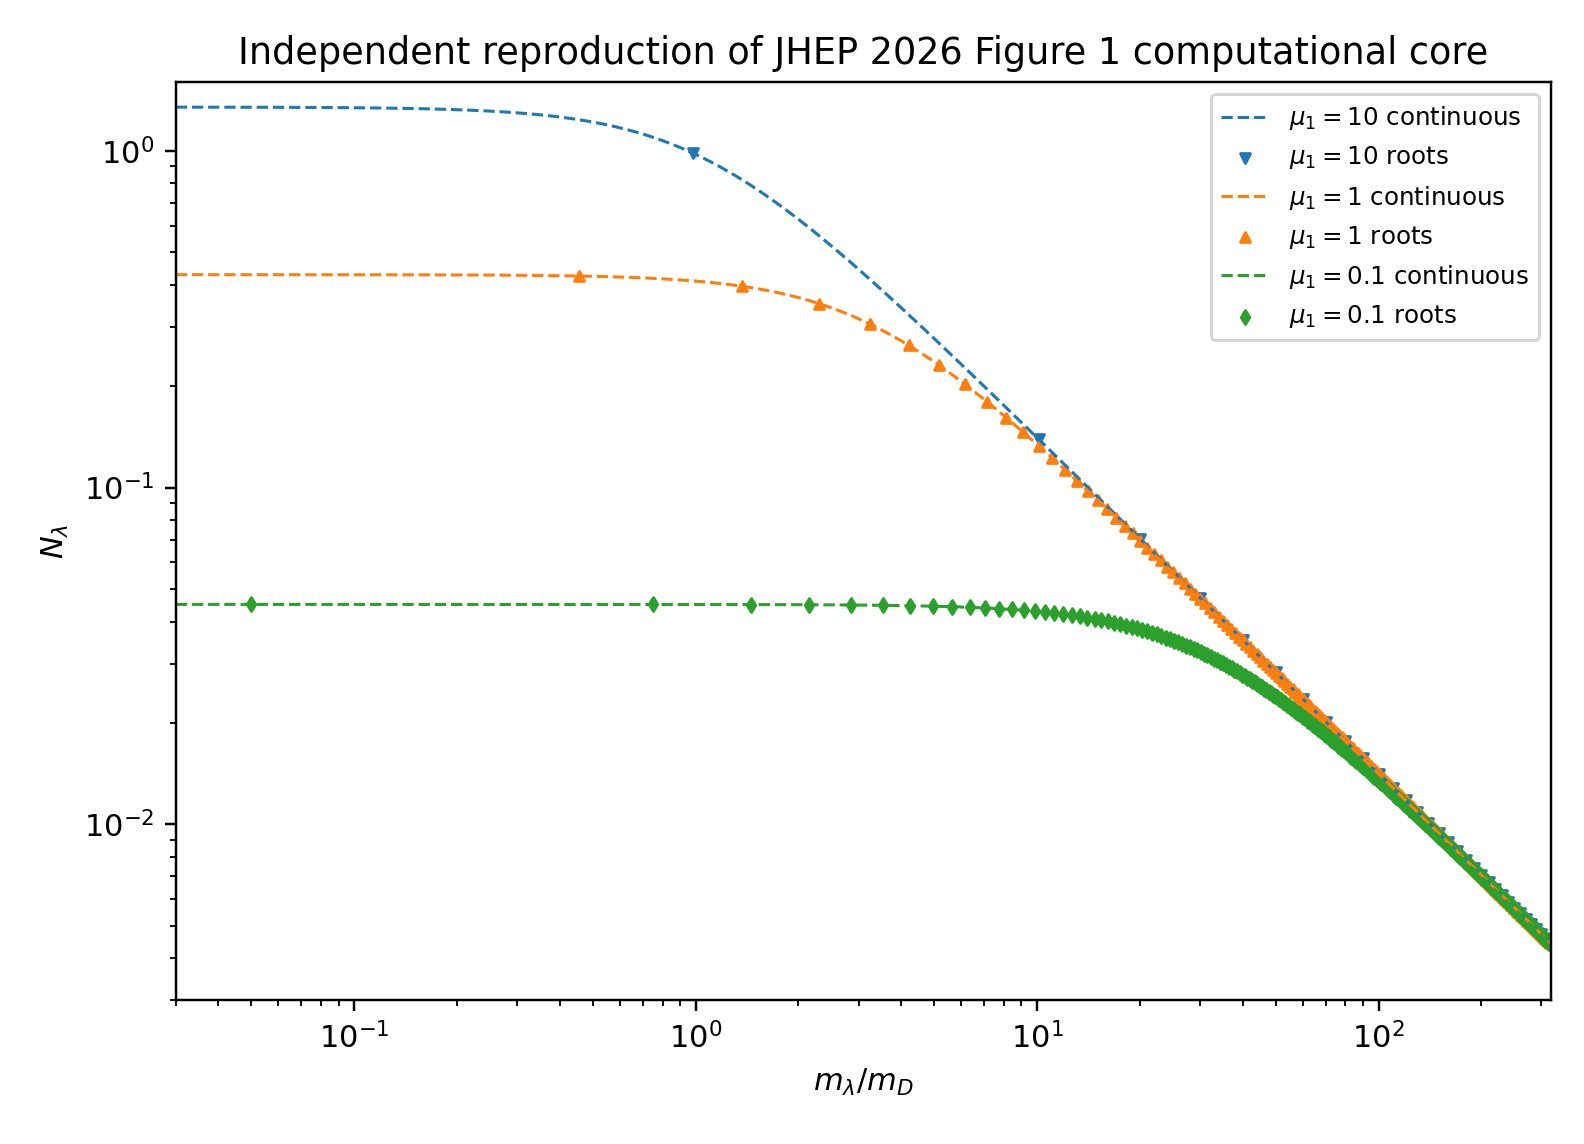
\includegraphics[width=0.98\linewidth]{figures/fig1_brane_dirac_replica.png}
\caption{Independent reproduction of the computational core of the target article's Figure~1. Dashed curves evaluate the published infinite-tower normalisation continuously; markers show independently solved physical roots for $m_D=1$ and $\mu_1=10,1,0.1$. This figure was generated from the published equations and is not copied from the target article.}
\label{fig:fig1-replica}
\end{figure}

\subsection{Conditioning-aware validation of all plotted roots}\label{sec:conditioning}

The first implementation included an additional raw equation-residual gate, $|F(y)|<10^{-9}$, for every plotted root of
\begin{equation}
F(y)=\pi\cot(\pi y)-\left(\frac{\mu_1}{m_D}\right)^2y.
\end{equation}
That gate failed because the maximum raw residual was $2.67\times10^{-6}$. This automatic failure is preserved in the audit trail; it was not silently overwritten.

A subsequent conditioning audit showed that the raw function residual is a poor coordinate-error metric near cotangent poles, where $|F'(y)|$ is large. We therefore evaluated the first-order backward coordinate error $|F/F'|$ for all 3552 plotted roots and normalized it by the already requested Brent coordinate tolerance, $\mathrm{xtol}+\mathrm{rtol}|y|$. All 3552 roots lie within that requested coordinate tolerance. The maximum normalized error is $0.250095$, the median is $0.002510$, and the 99th percentile is $0.239561$.

The root with the largest raw residual, at $\mu_1=10$, $n=30$, was independently re-solved at 80-digit precision; its mass differed from the double-precision result by $2.90\times10^{-12}$. A second 80-digit check at the root with the largest normalized backward error differed by $2.73\times10^{-12}$ in mass. No replacement raw-residual threshold was introduced. The original gate is therefore interpreted as a technical diagnostic failure caused by conditioning, while the Figure~1 root coordinates remain numerically validated.

\section{Attempted extension to Figure~5}\label{sec:figure5}

\subsection{Direct contour digitization}\label{sec:digitization}

The target article's Figure~5 gives $90\%$ confidence contours for the Dirac-brane scenario, with solid curves corresponding to Daya Bay and dotted curves to MINOS/MINOS+ \autocite{degiorgi2026}. Four Daya Bay points were selected for a direct test: normal and inverted ordering at $m_{\rm lightest}=0.3$ and $1.0$~eV. The published curves were digitized from the version-of-record PDF using multiple raster resolutions and color-threshold variants. All four points passed the frozen digitization QA.

\begin{table}[H]
\centering
\caption{Direct Figure~5 digitization and local open-comparator outcome. ``Minimum crossings'' is a certified lower bound within the digitization interval at $N=192$.}
\label{tab:fig5}
\begin{tabular}{@{}lcccc@{}}
\toprule
Ordering & $m_{\rm lightest}$ [eV] & $1/R$ median [$\mu$m$^{-1}$] & Digitization interval & Minimum crossings \\
\midrule
NO & 0.3 & 51.2746  & 51.1204--51.3168   & 2 \\
NO & 1.0 & 172.6645 & 171.4732--173.7360 & 2 \\
IO & 0.3 & 54.3497  & 54.2921--54.3824   & 2 \\
IO & 1.0 & 180.0192 & 179.9481--180.8174 & 3 \\
\bottomrule
\end{tabular}
\end{table}

In every case, the open comparator crosses the project threshold $\Delta\chi^2=4.605170185988092$ multiple times within the narrow digitization interval. Therefore none of the four points defines a unique pointwise replication candidate. The correct interpretation is \emph{local numerical topology unresolved in the open comparator}; it is not evidence that the published contour is wrong or non-replicable.

\subsection{Correction of an earlier topology attribution}\label{sec:d28a}

An earlier version of the audit reported 39 threshold crossings for $N=192$ and 17 for $N=384$. Reviewer-style inspection identified a confound: the two truncations had been evaluated on different radius-grid densities. A matched-grid rerun withdrew that interpretation. On common grids, the crossing counts increased from 65/67 at 318 points to 199/203 at 635 points and 331/333 at 1269 points for $N=192/384$, respectively. Neither truncation was internally stable under radius-grid refinement. At the finest common grid, however, the two $\Delta\chi^2$ curves were nearly identical pointwise (Pearson correlation $0.9999988$; median absolute difference $0.0129$). The earlier claim of KK-truncation-dependent micro-topology is therefore not retained.

\section{Public Daya Bay control and correction of the calibration claim}\label{sec:dayabay-control}

The Daya Bay Collaboration has released the full 3158-day data set and states that the public material is sufficient to reproduce the standard oscillation-parameter measurement \autocite{dayabay2023,dayabaydata2025}. The public software stack separates the model from the analysis scripts; this distinction matters for interpreting the earlier audit.

The public covariance-fit reference has $\chi^2=557.9755550235543$. Running the public full-fit route in the same frozen software environment reproduced that value as $557.9755550235410$, an absolute difference of $1.33\times10^{-11}$. All 21 best-fit parameters were reproduced to a maximum absolute difference of $5.77\times10^{-11}$.

By contrast, the project's earlier fixed-oscillation profile over 19 spectrum-shape parameters returned $\chi^2=574.1120550199523$, identical to the archived worker result but $16.1365$ above the public full-fit reference. The correct conclusion is not that the Daya Bay public model failed calibration. Rather, the fixed-coordinate profiling procedure was computationally reproducible but not equivalent to the public full-fit procedure. Earlier project-defined binary thresholds on absolute $\chi^2$, Spearman correlation, and $\Delta\Delta\chi^2$ summaries are retained only as historical audit diagnostics and are not used as scientific pass/fail criteria in this manuscript.

\section{Reproducibility status and external continuous integration}\label{sec:reproducibility}

The current Figure~1 replication is publicly available at the frozen repository revision
\href{https://github.com/yokken0907/led-neutrino-open-reproduction-audit/tree/73728590833e10c85eb2dd75bf844b825271b53d}{\texttt{73728590833e}}. The repository contains the independent D29A Figure~1 calculation, the D29B conditioning-aware validator, an exact Python environment, and the one-command runner \texttt{reproduce\_figure1.sh}.

The same frozen revision was executed independently on GitHub-hosted Ubuntu in
\href{https://github.com/yokken0907/led-neutrino-open-reproduction-audit/actions/runs/36403948683}{workflow run 36403948683}. The hosted runner reported Ubuntu~24.04.5 and Python~3.12.14. The workflow reproduced the deliberately preserved D29A automatic raw-residual failure, all nine successful finite/infinite triangulation checks, all three $>99\%$ unitarity checks, and the final D29B verdict
\texttt{PASS\_FIGURE1\_COMPUTATIONAL\_CORE\_INDEPENDENT\_REPLICATION\_AFTER\_CONDITIONING\_AUDIT}. The CI verification step completed with \texttt{FIGURE1\_REPLICATION\_CI\_PASS}.

The uploaded workflow artifact is ID~10962090038; GitHub reported SHA-256
\texttt{9f0d1b782f9995f2c4379446e5af4c7aadb46c375a7096b66610dba36823cea3}. The artifact contains the D29A and D29B result JSON files, the three root tables, and the independently generated Figure~1-style spectrum. This external run therefore tests the current manuscript-facing replicated subset rather than only historical D25--D27 outputs.

\section{Limitations and claim boundaries}\label{sec:limitations}

The successful result is deliberately narrow. The present work establishes an independent reproduction of the Figure~1 Brane--Dirac computational spectrum from the published equations. It does not reconstruct the target authors' full numerical infrastructure, experimental likelihoods, or the published Figure~5 exclusion contours.

The Figure~5 comparator uses open experimental products and a related public implementation, not the target authors' unavailable likelihood pipeline. Multiple local threshold crossings in that comparator therefore diagnose the open reconstruction, not the original article. The target paper's experiment-level results are neither validated nor falsified here.

The conditioning correction after the initial D29A automatic failure is also explicitly bounded. The original raw-residual failure is retained in the audit trail. The later correction does not loosen that residual threshold; it demonstrates that raw residual magnitude is ill-conditioned as a root-coordinate accuracy metric near cotangent poles and validates the roots against the solver-coordinate tolerance and two high-precision calculations.

The reviewer-runnable Figure~1 workflow is now public and has passed a clean GitHub-hosted Ubuntu execution at the frozen revision given in Section~\ref{sec:reproducibility}. This establishes reproducibility of the manuscript-facing computation, while ordinary ReScience review still determines whether the demonstrated subset is sufficiently substantial for publication.

\section{Conclusion}\label{sec:conclusion}

The Brane--Dirac spectrum underlying Figure~1 of de Giorgi, Pasari, and Turner was independently reproduced from the published equations. Two independent numerical routes agree at nine preregistered anchors to at worst $1.29\times10^{-9}$ in mass, and the target article's $>99\%$ unitarity criterion is satisfied for all three published $\mu_1$ choices. A conditioning-aware audit over 3552 roots and two 80-digit checks resolves an initially failed raw-residual diagnostic without changing the physical calculation.

The replication does not extend to the selected Figure~5 exclusion points: the tested open comparator has multiple local threshold crossings inside each digitization interval, so a unique pointwise mapping to the published contour is not established. A separate public Daya Bay control reproduces the covariance-fit reference to numerical precision and shows that an earlier fixed-coordinate profiling route was non-equivalent rather than a failure of the public reference analysis.

The resulting claim is therefore bounded but positive: \textbf{Figure~1 is the successfully replicated computational subset; Figure~5 remains unresolved in the open reconstruction.} The \texttt{[Re]} classification is restricted to that Figure~1 subset and remains subject to the ordinary ReScience C editorial and reviewer standard.
